%%%%%%%%%%%%%%%%%%%%%%%%%%%%%%%%%%%%%%%%%%%%%%%%%
%%%%%%%%%%%%%%%%%%%%%%%%%%%%%%%%%%%%%%%%%%%%%%%%%
%% File: nopadon_cmu_dissertation.tex
%% Author: Nopadon Juneam
%% Date:  May 4, 2017
%% Email: juneam.n@gmail.com, nopadon_j@cmu.ac.th
%% Department of Computer Science, Chiang Mai University
%%
%% This is the main tex file of the latex template for Thesis and Dissertation for Chiang Mai University.
%% The propose of the tex file is to demonstrate the use of CMU Thesis & Dissertation Package for writing a %% thesis/dissertation according to the format of the graduate school of Chiang Mai University.
%%
%% Caution: Please keep in mind that the file is not the official template from the graduate school of 
%% Chiang Mai University. However, the author's dissertation using this tex file have passed the school's 
%% inspection (in April 2017).
%%
%% Credit: This main tex file is modified from the original latex template for Theses and Dissertation of 
%% Chulalongkorn University by Dr. Nattee Niparnan.
%%
%% The file is compatible with XeLaTex and tested with TeX Live 2016 Version 3.14159265.
%% 
%% You can freely modify the file.
%%%%%%%%%%%%%%%%%%%%%%%%%%%%%%%%%%%%%%%%%%%%%%%%%
%%%%%%%%%%%%%%%%%%%%%%%%%%%%%%%%%%%%%%%%%%%%%%%%%

%%-------------------------------------------------------------------------------
%%-                               PREAMBLE                                          - 
%%-------------------------------------------------------------------------------
\documentclass[a4paper,12pt,engthesis,doctor]{chiangmai}
%% These are some useful LaTeX package
%% the list is taken from the bare_jnrl.tex of IEEEtran, by Michael Shell
%\usepackage[pdftex]{graphicx}           % for including graphics (eps and pdf)
%% NOTE: for dual use with latex and pdflatex, instead load graphicx like:
% \ifx\pdfoutput\undefined
%  \usepackage[dvips]{graphicx}
%  \graphicspath{{./figure/}}
% \else
%  \usepackage[pdftex]{graphicx}
%  \graphicspath{{./figure/}}
% \fi
\graphicspath{{./figure/}}


\usepackage{amssymb}
\usepackage[normalem]{ulem}
\usepackage[cmex10]{amsmath}	% math package provides several command and symbols
                                				% cmex10 option force only type 1 font to be used
\interdisplaylinepenalty=2500   		% amsmath set this value to 10000, if you want to adjust
                                				% this, do so after use the package
                                
\usepackage{newalg}			% package for writing a pseudo code
\usepackage{array}				% improvement to the tabular and array
%\usepackage{mdwmath}			% other useful math package for formating equations
%\usepackage{mdwtab}
\usepackage{subfig}				% for placing subfigures in one figures environment
                                				% (for example, Fig 1a and 1b)
\usepackage{url}				% for breaking urls (use \url{http://www.example.com}

%\usepackage{times}             		% for times roman font
%\usepackage{lscape}			% for landscape page
\usepackage{lipsum}  			% for generating dummy texts

\usepackage{background}			% for CMU watermark background
\backgroundsetup{				% Comment to disable watermark
scale=1.1,
angle=0,
opacity=0.5,
hshift=25pt,
contents={
\includegraphics[width=\paperwidth,height=\paperheight]{figures/copyrights.jpg}}
}

\usepackage{multirow}
\usepackage{enumitem}
\usepackage{bibentry}
\usepackage{etoolbox}

\AtBeginEnvironment{definition}{\renewcommand\eminnershape{\normalfont \bfseries}}
\AtBeginEnvironment{theorem}{\renewcommand\eminnershape{\normalfont \itshape}}
\AtBeginEnvironment{lemma}{\renewcommand\eminnershape{\normalfont \itshape}}
\AtBeginEnvironment{corollary}{\renewcommand\eminnershape{\normalfont \itshape}}
\AtBeginEnvironment{proposition}{\renewcommand\eminnershape{\normalfont \itshape}}

%% Environment, theorem, etc.
\newtheorem{theorem}{Theorem}[chapter]
\newtheorem{corollary}[theorem]{Corollary}
\newtheorem{lemma}[theorem]{Lemma}
\newtheorem{proposition}[theorem]{Proposition}
\newtheorem{definition}[theorem]{Definition}

\usepackage{graphicx}
\usepackage{color}
\definecolor{light-gray}{gray}{0.5}
\usepackage{array}
\newcolumntype{L}[1]{>{\raggedright\let\newline\\\arraybackslash\hspace{0pt}}m{#1}}
\newcolumntype{C}[1]{>{\centering\let\newline\\\arraybackslash\hspace{0pt}}m{#1}}
\newcolumntype{R}[1]{>{\raggedleft\let\newline\\\arraybackslash\hspace{0pt}}m{#1}}
\usepackage{multirow}

% we use \mathbb{R} instead of \Re
\renewcommand{\Re}{\mathbb{R}}

\newcommand{\pspan}{\mbox{\sc span}^+}
\newcommand{\nspan}{\mbox{\sc span}^-}
\newcommand{\itr}{\mbox{\sc int}}
\newcommand{\co}{\mbox{\sc co}}
\newcommand{\ri}{\mbox{\sc ri}}
\newcommand{\ints}{\Omega}
\newcommand{\rspace}{\Re^3}
\newcommand{\ha}{\mathcal{H}}
\newcommand{\FindInts}{\mbox{\sc FindInts}}
\newcommand{\FindFG}{\mbox{\sc FindFG}}
\newcommand{\La}{\mathcal{U}}
\newcommand{\Lb}{{}^S\mathcal{U}}
\newcommand{\Lc}{{}^\mathfrak{F}\mathcal{U}}
\newcommand{\Ta}{\mathcal{P}}

%% For proof
\def\QED{\mbox{\rule[0pt]{1.3ex}{1.3ex}}}	% for a filled box
\def\proof{\vspace*{-5mm}\noindent{\itshape Proof: }}
\def\endproof{\hspace*{\fill}~\QED\par\endtrivlist\unskip\par}

%% Correct bad hyphenation here
\hyphenation{net-works physico-mi-metics kij-sirikul cha-lerm-ek inta-nagon-wiwat tiny-os reducibiliti-es sequen-tial polylog-arithmic}

%%------------------------------------------------------------
%%-         SETTING THESIS PARAMETERS     -
%%------------------------------------------------------------

\thesistitle					% set the thesis tile (use {\wbr} for word break)
{หัวข้อดุษฎีนิพนธ์} %Thai Title
{Dissertation Title} %English title (auto upper case)

\authortitle					% set the title of the author, e.g., Mr., Miss, Dr. etc.
{นาย} % Thai Title of the author
{Mr.} % English Title of the author
\thesisauthor				% set the author name (must not include title (Mr., Miss, Dr., etc.)
{ชื่อ นามสกุล} % Author name in Thai
{Name Surname} % Author name in English

\advisor					% set the advisor
{รองศาสตราจารย์ ดร. ชื่อ นามสกุล} % Advisor name in Thai
{รศ. ดร. ชื่อ นามสกุล} % Advisor name in Thai with abbrev. title
{Assoc. Prof. Dr. Name Surname} % Advisor name in English
{ASST. PROF. NAME  URNAME, Ph.D.} % Advisor name in English with abbrev. title 	
									      % (Capital letters except Ph.D.))

%% If the thesis has co-advisor, use this optional command
\firstcoadvisor
{ศาสตราจารย์ ดร. ชื่อ นามสกุล}  % Co-Advisor name in Thai
{ศ. ดร. ชื่อ นามสกุล}  % Co-Advisor name in Thai with abbrev. title
{Prof. Dr. Name Surname} % Co-Advisor name in English
{PROF. DR. NAME SURNAME, Ph.D.} % Co-Advisor name in English with abbrev. title 
							             % (Capital letters except Ph.D.))
\secondcoadvisor
{รองศาสตราจารย์ ดร. ชื่อ นามสกุล}  % Co-Advisor name in Thai
{รศ. ดร. ชื่อ นามสกุล}  % Co-Advisor name in Thai with abbrev. title
{Assoc. Prof. Dr. Name Surname} % Co-Advisor name in English 
{ASSOC. PROF. DR. NAME SURNAME, Ph.D.} % Co-Advisor name in English with abbrev. title 
							                    % (Capital letters except Ph.D.))

\faculty					% set the faculty
{วิทยาศาสตร์} % Name of the faculty in Thai
{Science} % Name of the faculty in English
\department				% set the department
{วิทยาการคอมพิวเตอร์} % Name of the department in Thai
{Computer Science} % Name of the department in English
\fieldofstudy				% set the field of study 
{วิทยาการคอมพิวเตอร์} % Field in Thai
{Computer Science} % Field in English
\degree					% set the degree name
{วิทยาศาสตร์ดุษฎีบัณฑิต} % Degree name in Thai
{Doctor of Philosophy} % Degree name in English
\examdate{3}{May}{2017} % Thesis defense date (A.D. calendar)

\committee				% list of committee, please use \CommitteeBlock,
{
\CommitteeBlock{Chairman}{Asst. Prof. Dr. Name Surname} % Chairman
\CommitteeBlock{Member}{Asst. Prof. Dr. Name Surname} % Examiner
\CommitteeBlock{Member}{Assoc. Prof. Dr. Name Surname} % Examiner
\CommitteeBlock{Member}{Assoc. Prof. Dr. Name Surname} % Examiner
\CommitteeBlock{Member}{Assoc. Prof. Dr. Name Surname} % Examiner
}

%% DedicationTitle
\dedicationTitle{To ... \\ (Whom I would like to \\ Dedicate to) ...}

\def\vect#1{\mbox{\boldmath $#1$}}
%\def\vect#1{{\bf #1}}
\def\mat#1{{\cal #1}}
\def\lvect#1{\overrightarrow{#1}}
\def\bfrac#1#2{\frac{\displaystyle\strut #1}{\displaystyle\strut #2}}
\def\RR{\hbox{I\kern-.2em\hbox{R}}}
\def\eqdef{\buildrel \rm def \over =}
\def\arg{{\rm Arg}}
\def\range{{\rm range}}
\def\va{\vect{a}}
\def\vb{\vect{b}}
\def\vc{\vect{c}}
\def\ve{\vect{e}}
\def\vd{\vect{d}}
\def\vf{\vect{f}}
\def\vg{\vect{g}}
\def\vk{\vect{k}}
\def\vm{\vect{m}}
\def\vn{\vect{n}}
\def\vw{\vect{w}}
\def\vp{\vect{p}}
\def\vo{\vect{o}}
\def\vq{\vect{q}}
\def\vr{\vect{r}}
\def\vs{\vect{s}}
\def\vt{\vect{t}}
\def\vuu{\vect{\omega}}
\def\vu{\vect{u}}
\def\vv{\vect{v}}
\def\vx{\vect{x}}
\def\vy{\vect{y}}
\def\vz{\vect{z}}
\def\vF{\vect{F}}
\def\vM{\vect{M}}
\def\mA{\mat{A}}
\def\mC{\mat{C}}
\def\mD{\mat{D}}
\def\mE{\mat{E}}
\def\mG{\mat{G}}
\def\mP{\mat{P}}
\def\mL{\mat{L}}
\def\mR{\mat{R}}
\def\mF{\mat{F}}
\def\mS{\mat{S}}
\def\mV{\mat{V}}
\def\mH{\mat{H}}
\def\mJ{\mat{J}}
\def\mI{\mat{I}}
\def\mm{\mat{M}}
\def\mt{\mat{T}}
\def\mT{\mat{T}}
\def\mK{\mat{K}}
\def\mW{\mat{W}}
\def\atz{|_{0,0}}
\def\w{\vect{w}}
\def\aa#1{\hspace{-#1}\psfig{width=16pt,figure=a.ill}\hspace{#1}\hspace{-16pt}}
\def\bb#1{\hspace{-#1}\psfig{width=16pt,figure=b.ill}\hspace{#1}\hspace{-16pt}}
\def\cc#1{\hspace{-#1}\psfig{width=16pt,figure=c.ill}\hspace{#1}\hspace{-16pt}}
\def\dd#1{\hspace{-#1}\psfig{width=16pt,figure=d.ill}\hspace{#1}\hspace{-16pt}}
\def\ee#1{\hspace{-#1}\psfig{width=16pt,figure=e.ill}\hspace{#1}\hspace{-16pt}}
\def\ff#1{\hspace{-#1}\psfig{width=16pt,figure=f.ill}\hspace{#1}\hspace{-16pt}}
\def\gg#1{\hspace{-#1}\psfig{width=16pt,figure=g.ill}\hspace{#1}\hspace{-16pt}}
\def\hh#1{\hspace{-#1}\psfig{width=16pt,figure=h.ill}\hspace{#1}\hspace{-16pt}}
\def\ii#1{\hspace{-#1}\psfig{width=16pt,figure=i.ill}\hspace{#1}\hspace{-16pt}}
%%-------------------------------------------------------------------------------
%%-                               DOCUMENT                                      -
%%-------------------------------------------------------------------------------
\begin{document}
%% Thesis starts with Front Cover
\makefrontcover

%% Fly Leaf
\newpage~\thispagestyle{empty}

%% Inner Cover
\makeinnercover

%% Title Page
\maketitlepage

%% Approval Page
\makeapprovalpage

%% Dedication Page
\makededicationpage

%% Acknowledgement
\begin{acknowledgements}
\setlength{\parskip}{12pt}
\setlength{\parindent}{10mm}
\onehalfspacing

\lipsum[1-3] % dummy texts

\begin{spacing}{4}
\end{spacing}
\hfill Name and Surname of the author
\end{acknowledgements}


%% Abstract in Thai
\begin{thaiabstract}
\setlength{\parskip}{12pt}
\setlength{\parindent}{10mm}
\begin{spacing}{1.5}
\fontsize{16}{19.2}\selectfont
%% dummy texts in Thai
เนื้อหาจำลองแบบเรียบๆ ที่ใช้กันในธุรกิจงานพิมพ์หรืองานเรียงพิมพ์ มันได้กลายมาเป็นเนื้อหาจำลองมาตรฐานของธุรกิจดังกล่าวมาตั้งแต่ศตวรรษที่ 16 เมื่อเครื่องพิมพ์โนเนมเครื่องหนึ่งนำรางตัวพิมพ์มาสลับสับตำแหน่งตัวอักษรเพื่อทำหนังสือตัวอย่าง เนื้อหาจำลองแบบเรียบๆ ที่ใช้กันในธุรกิจงานพิมพ์หรืองานเรียงพิมพ์ มันได้กลายมาเป็นเนื้อหาจำลองมาตรฐานของธุรกิจดังกล่าวมาตั้งแต่ศตวรรษที่ 16 เมื่อเครื่องพิมพ์โนเนมเครื่องหนึ่งนำรางตัวพิมพ์มาสลับสับตำแหน่งตัวอักษรเพื่อทำหนังสือตัวอย่าง เนื้อหาจำลองแบบเรียบๆ ที่ใช้กันในธุรกิจงานพิมพ์หรืองานเรียงพิมพ์ มันได้กลายมาเป็นเนื้อหาจำลองมาตรฐานของธุรกิจดังกล่าวมาตั้งแต่ศตวรรษที่ 16 เมื่อเครื่องพิมพ์โนเนมเครื่องหนึ่งนำรางตัวพิมพ์มาสลับสับตำแหน่งตัวอักษรเพื่อทำหนังสือตัวอย่าง
\normalsize
\end{spacing}
\end{thaiabstract}


%% Abstract in Englosh
\begin{englishabstract}
\setlength{\parskip}{12pt}
\setlength{\parindent}{10mm}
\onehalfspacing
\lipsum[1-2] % dummy texts
\end{englishabstract}


%% Table of Content
\tolerance=1000 
\tableofcontents  

%% List of Tables      
\listoftables

%% List of Figures
\listoffigures          

%% List of Abbreviations
\begin{listabbv}
\setlength{\parskip}{12pt}
\setlength{\parindent}{10mm} 
\onehalfspacing
%% dummy texts
\begin{tabular}{@{}p{10mm}@{}p{2.5cm}@{}p{11.5cm}}	
    & \textsc{RAM} & Random Access Machine. \vspace*{3mm} \\   
    & \textsc{CD-RW} & Compact Disc Rewritable. \vspace*{3mm}  
\end{tabular} 
\end{listabbv}


%% List of Symbols
\begin{listsymbol}
\setlength{\parskip}{12pt}
\setlength{\parindent}{10mm} 
\onehalfspacing
%% dummy texts
\begin{tabular}{@{}p{10mm}@{}p{2.5cm}@{}p{11.5cm}}
    & $\leq$ & Less than or equal to. \vspace*{3mm} \\
    & $=$    & Equal to. \vspace*{3mm} \\
    & $\geq$ & Greater than or equal to. \vspace*{3mm} \\
\end{tabular}
\end{listsymbol}


%% Statements of Originality in Thai
\begin{statementthai}
\setlength{\parskip}{12pt}
\setlength{\parindent}{10mm}
\begin{spacing}{1.5}
\normalsize

\begin{enumerate}[leftmargin=*, labelsep=6.5mm] 

\item \fontsize{16}{19.2}\selectfont เนื้อหาจำลองแบบเรียบๆ ที่ใช้กันในธุรกิจงานพิมพ์หรืองานเรียงพิมพ์ มันได้กลายมาเป็นเนื้อหาจำลองมาตรฐานของธุรกิจดังกล่าวมาตั้งแต่ศตวรรษที่ 16

\item เนื้อหาจำลองแบบเรียบๆ ที่ใช้กันในธุรกิจงานพิมพ์หรืองานเรียงพิมพ์ มันได้กลายมาเป็นเนื้อหาจำลองมาตรฐานของธุรกิจดังกล่าวมาตั้งแต่ศตวรรษที่ 16


\end{enumerate}
\normalsize
\end{spacing}
\end{statementthai}


%% Statements of Originality in English
\begin{statementenglish}
\setlength{\parskip}{12pt}
\setlength{\parindent}{10mm}
\onehalfspacing
\begin{enumerate}[leftmargin=*, labelsep=6.5mm] 
\item \lipsum[2-2] % dummy texts

\item \lipsum[2-2] % dummy texts

\end{enumerate}
\end{statementenglish}


%% Empty Page to set new margin
\clearpage~\thispagestyle{empty}
\setlength{\voffset}{-1in+25mm}
\setlength{\textheight}{23.70cm} 

%%-----------------------------------------------------------------------------
%%-                               MAIN CONTENT                               -
%%-----------------------------------------------------------------------------
%% Chapter 1
\chapter{Introduction}
\setlength{\parskip}{12pt}
\setlength{\parindent}{10mm} 
\onehalfspacing
\lipsum[1-3] % dummy texts

\section{Historical Background}
\lipsum[1-3] % dummy texts

\section{Literature Review}
\lipsum[1-3] % dummy texts

\section{Theory and/or Principles}
\lipsum[1-3] % dummy texts

\section{Scope of Study}
\begin{enumerate}
\item \lipsum[2-2] % dummy texts
\item \lipsum[2-2] % dummy texts
\item \lipsum[2-2] % dummy texts
\end{enumerate}



 

%% Chapter 2
\chapter{Contents}
\setlength{\parskip}{12pt}
\setlength{\parindent}{10mm} 
\onehalfspacing

The goal of this chapter is to illustrate the environments for definition, lemma, theorem, corollary, proof, figure, and table.

\section{Definition, Lemma, Theorem, Corollary, and Proof}
Let $\mathbb{N} = \{1, 2, 3, \ldots \}$ be the set of natural numbers.

\begin{definition}[Prime and Composit]
\label{primes and composits}
A natural number is called a {\em prime number} (or a {\em prime}) if it has exactly two positive divisors, $1$ and the number itself \cite{numbertheory-underwoord}.  Natural numbers greater than $1$ that are not prime are called {\em composite}.
\end{definition}

\begin{lemma}[2 is prime]
\label{2-is-prime} 
2 is a prime number.
\end{lemma}

\begin{proof}
2 and 1 are exactly two positive divisors of 2.
\end{proof}

\begin{theorem}[2 is the only even prim number]
\label{2-is-prime} 
An even natural number greater than 2 is not prime.
\end{theorem}

\begin{proof}
Every even natural number is a composite as there are at least three positive divisors: $1$, $2$, and the number itself.
\end{proof}

From Theorem \ref{2-is-prime}, we have the following corollary.

\begin{corollary}[Most of even natural numbers are not prime]
$2$ is the only even prime number.
\end{corollary}

\section{Table and Figure}
Figure \ref{prime-distribution} illustrates the asymtotic distribution of prime numbers according to the \textsc{Prime Number Theorem (PNT)} which is stated as follows:

\begin{theorem}[\textsc{Prime Number Theorem (PNT)}]
Let $\pi(x)$ denote the prime-counting function that gives the number of primes less than or equal to $x$, for any real number $x$.

\[ \lim_{x \to \infty} \frac{\pi(x)}{\frac{x}{\log{(x)}}} = 1\]
\end{theorem}

In other words, the \textsc{PNT} states that $x / \log{x}$ is a good approximation to $\pi(x)$.

\begin{figure}[h!] \vspace{10pt} \centering
\vspace{7pt}
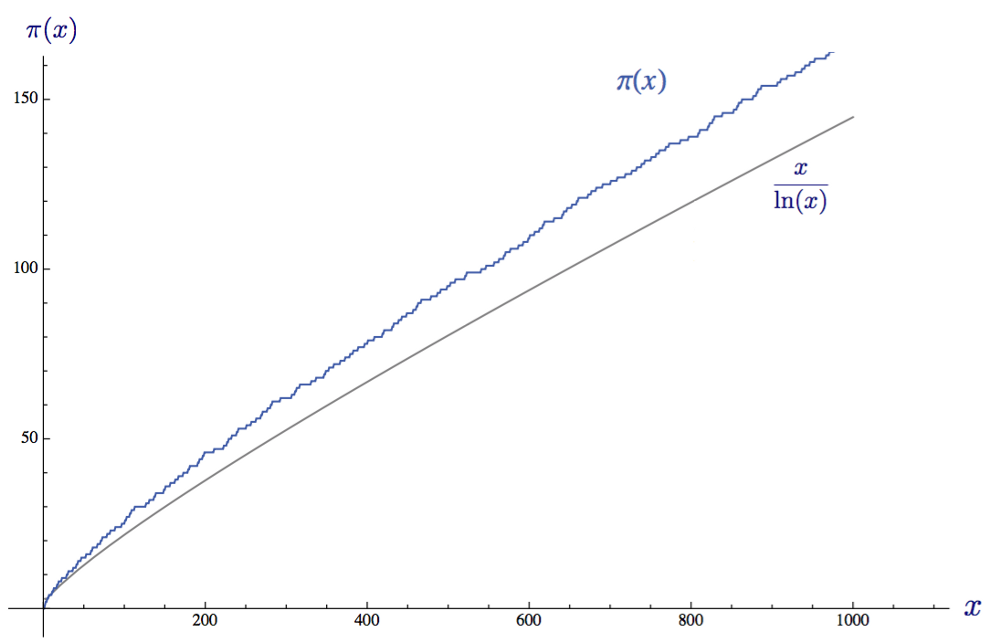
\includegraphics[width=10cm]{figures/prime-number-theorem-absolute.png}
\vspace{7pt}
\caption[Distribution of prime numbers regarding Prime Number Theorem ]{The prime counting function $\pi(x)$ and the estimate from the the \textsc{PNT} plotted up to $x$ = 1000. Source: \url{https://cdn-images-1.medium.com/max/1000/1*AhZ7SxlQWrBGd4HXHs1JWA.png}}
\label{prime-distribution}
\vspace{-5mm}
\end{figure}

The following table shows all prime numbers up to 1000.

\begin{table}[h!]
\vspace{-2mm}
\begin{center}
\caption[All prime numbers up to 1000.]{All prime numbers up to 1000.}
\begin{tabular}{| c | c | c | c | c | c | c | c | c | c |}
\hline
& 2 & 3 & 5 & 7 & 11 & 13 & 17 & 19 & 23 \\
29 & 31 & 37 & 41 & 43 & 47 & 53 & 59 & 61 & 67 \\
71 & 73 & 79 & 83 & 89 & 97 & 101 & 103 & 107 & 109 \\
113 & 127 & 131 & 137 & 139 & 149 & 151 & 157 & 163 & 167 \\
173 & 179 & 181 & 191 & 193 & 197 & 199 & 211 & 223 & 227 \\
229 & 233 & 239 & 241 & 251 & 257 & 263 & 269 & 271 & 277 \\
281 & 283 & 293 & 307 & 311 & 313 & 317 & 331 & 337 & 347 \\
349 & 353 & 359 & 367 & 373 & 379 & 383 & 389 & 397 & 401 \\
409 & 419 & 421 & 431 & 433 & 439 & 443 & 449 & 457 & 461 \\
463 & 467 & 479 & 487 & 491 & 499 & 503 & 509 & 521 & 523 \\
541 & 547 & 557 & 563 & 569 & 571 & 577 & 587 & 593 & 599 \\
601 & 607 & 613 & 617 & 619 & 631 & 641 & 643 & 647 & 653 \\
659 & 661 & 673 & 677 & 683 & 691 & 701 & 709 & 719 & 727 \\
733 & 739 & 743 & 751 & 757 & 761 & 769 & 773 & 787 & 797 \\
809 & 811 & 821 & 823 & 827 & 829 & 839 & 853 & 857 & 859 \\
863 & 877 & 881 & 883 & 887 & 907 & 911 & 919 & 929 & 937 \\
941 & 947 & 953 & 967 & 971 & 977 & 983 & 991 & 997 & \\
\hline
\end{tabular}
\end{center}
\vspace{-7mm}
\end{table}







%% Chapter 2
\chapter{Conclusion and Suggestion}
\setlength{\parskip}{12pt}
\setlength{\parindent}{10mm} 
\onehalfspacing
\label{conclusion}

\lipsum[1-7] % dummy texts



%% Empty Page to reset margin
\setlength{\voffset}{-1in+35mm}
\setlength{\textheight}{22.70cm}
\clearpage~\thispagestyle{empty}

%% Bibliography
\bibliographystyle{abbrv}
\insertbibtoc
\bibliography{main} % speficy your bibtex file here (this example is main.bib).
\nobibliography* 

%%-----------------------------------------------------------------------------
%%-                               BACK SECTION                                -
%%-----------------------------------------------------------------------------

%% List os publications
\begin{listpublication}
\setlength{\parskip}{12pt}
\setlength{\parindent}{10mm} 
\onehalfspacing

\noindent
\begin{enumerate}[label={\theenumi)}, labelsep=6.5mm, leftmargin=20mm]
\item Authors' name. Publication title,  {\em Journal/Conference}, Vol. $\ldots$, Month and year of publication, Page No. $\ldots$.
\item Authors' name. Publication title,  {\em Journal/Conference}, Vol. $\ldots$, Month and year of publication, Page No. $\ldots$.
\item Authors' name. Publication title,  {\em Journal/Conference}, Vol. $\ldots$, Month and year of publication, Page No. $\ldots$.
\item Authors' name. Publication title,  {\em Journal/Conference}, Vol. $\ldots$, Month and year of publication, Page No. $\ldots$.

\end{enumerate}


\end{listpublication}


%% Curriculum Viate
\begin{cv}
\setlength{\parskip}{12pt}
\setlength{\parindent}{10mm} 
\onehalfspacing
\noindent
\begin{tabular}{@{}p{3cm}@{}p{12cm}}
    Author's Name & Mr. Name Surname \\
\end{tabular}    
\begin{spacing}{2}\end{spacing}

\noindent
\begin{tabular}{@{}p{3cm}@{}p{12cm}}
    Date of Birth & day month year \\
\end{tabular}    
\begin{spacing}{2}\end{spacing}

\noindent
\begin{tabular}{@{}p{3cm}@{}p{12cm}}
    Education &  Preious degree, Institute, City, Country, Year of graduation.
\end{tabular}    
\begin{spacing}{2}\end{spacing}

\noindent
\begin{tabular}{@{}p{3cm}@{}p{12cm}}
    Scholarship & Scholarship name, Granter, Duration of scholarship \\
\end{tabular}    
\begin{spacing}{2}\end{spacing}

\noindent
\begin{tabular}{@{}p{3cm}@{}p{12cm}}
    Publications  & Authors' name. Publication title,  {\em Journal/Conference}, Vol. $\ldots$, Month and year of publication, Page No. $\ldots$   \vspace*{0.3cm} \\
    	 		& Authors' name. Publication title,  {\em Journal/Conference}, Vol. $\ldots$, Month and year of publication, Page No. $\ldots$   \vspace*{0.3cm} \\
    		       
\end{tabular}
\begin{spacing}{2}\end{spacing}
\noindent
\begin{tabular}{@{}p{3cm}@{}p{12cm}}
Academic \par Experiences & \dotfill \\
	& \dotfill  
\end{tabular}     
\begin{spacing}{2}\end{spacing}
\noindent

\includegraphics[width=4cm]{figures/avatar.jpeg}
\end{cv}


\end{document}
